% Chapter Template

\chapter{PROPIEDADES MECANICAS DE UN BMG POROSO SINTERIZADO (NANOVIDRIOS)} % Main chapter title

\label{C5} % Change X to a consecutive number; for referencing this chapter elsewhere, use \ref{ChapterX}

\lhead{Capítulo 5. \emph{BMG POROSO SINTERIZADO (NANOVIDRIOS)}} % Change X to a consecutive number; this is for the header on each page - perhaps a shortened title


%----------------------------------------------------------------------------------------
%	SECTION 1
%----------------------------------------------------------------------------------------

\section{Introducción}
\label{S5_1}

En capítulos anteriores se ha explicado que las grandes deformaciones en vidrios metálicos se deben, normalmente,
al colapso de zonas de transformación de tensión cortante (STZ) que dan lugar a una o varias bandas de corte (SB).
Estas bandas de corte pueden provocar la falla frágil del material debido a la deformación heterogénea.
Para evitar la falla frágil es necesario controlar la deformación permanente del material, es decir, el comportamiento en el régimen elastoplástico.
Se han estudiado varias formas para lograr esto, y una de ellas ha sido la de obtener muestras de vidrio metálico con porosidad 
\citep{guan13,wang10,schuh07,liontas14}.

En el presente Capítulo, se estudiarán algunas características de los vidrios metálicos con porosidad. En la \sref{S5_2} se explicará
brevemente los fundamentos detrás del control de la deformación a través de la adición de poros.
Luego, en la \sref{S5_3}, se detallará el procedimiento utilizado para fabricar muestras de BMG Cu$_{46}$ Zr$_{54}$ con porosidad
(similar a las muestras de ``nanovidrios'' en otros experimentos y simulaciones \citep{adibi13,albe13}). Finalmente, en la \sref{S5_4},
se presentarán resultados de simulaciones
realizadas con Dinámica Molecular. Las simulaciones de la muestra sometida a esfuerzos uniaxiales nos permitirán analizar los poliedros
de Voronoi, las tensiones y deformaciones atómicas, así como también la forma en que la porosidad inicial afecta la deformación resultante
de la muestra.

%----------------------------------------------------------------------------------------
%	SECTION 1
%----------------------------------------------------------------------------------------

\section{Porosidad en Metales Cristalinos}
\label{S5_2}

En los metales cristalinos la deformación plástica está relacionada al concepto de dislocaciones. Las dislocaciones son imperfecciones lineales en
la red cristalina \citep{askeland98}, que distorsionan la perfección de la red. El movimiento de las dislocaciones (proceso llamado
\textit{deslizamiento}) es el que provoca la deformación plástica del material (véase \fref{C5:fg:dislocaciones}).

\begin{figure}[h!]
\centering
  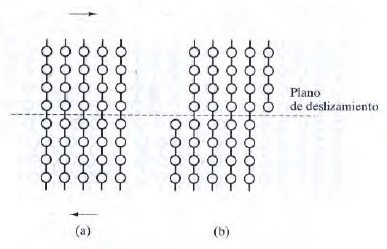
\includegraphics[width=10cm]{Cap_5/deslizamiento.png}
  \caption[Deslizamiento de un plano de átomos sobre otro plano adyacente]{Deslizamiento de un plano de átomos sobre otro plano adyacente
  (de \cite{shackelford04}, p. 203).}
  \label{C5:fg:dislocaciones}
\end{figure}

\cambio{Un material con dislocaciones es un material fácilmente deformable, puesto que habrán átomos débilmente enlazados con sus vecinos a lo largo del plano de deslizamiento. Por esto las redes cristalinas perfectas presentan una mayor resistencia.}

\cambio{Sin embargo, existen otros tipos de imperfecciones de la red, como por ejemplo los defectos puntuales, que dificultan el deslizamiento. Una imperfección de este estilo implica un estado de energía interna más alto, ya que los átomos en torno a dicha imperfección se encuentran ya sea en tensión o compresión, y por ello es necesario un esfuerzo externo mayor para superar esta ``barrera''.}

Estos conceptos sirven de fundamento del endurecimiento por solución (dónde se agregan átomos de otro material en una red) y el endurecimiento por deformación (se busca generar un ``bosque de dislocaciones'' que bloquee el deslizamiento), entre otras técnicas de aumento de la resistencia del material. 

Entre estas técnicas se incluye la adición de porosidad al material, motivo de estudio del presente capítulo. Se supone que, de igual manera que en los metales, los poros en vidrios metálicos limitan la propagación de bandas de corte y permiten una deformación más homogénea.

%----------------------------------------------------------------------------------------
%	SECTION 2
%----------------------------------------------------------------------------------------

\section{Preparación de la Muestra Porosa}
\label{S5_3}

Puesto que en el presente capítulo buscamos simular una muestra porosa, primero es necesario preparar dicha muestra. Para ello,
trataremos de \textbf{sinterizar} partículas de material, monitorizando constantemente la fracción de volumen sólido (en inglés \textit{Solid Volume Fraction} o SVF), para así detener el proceso cuando se haya alcanzado la porosidad deseada.

El sinterizado es un proceso durante el cual se aplica simultáneamente calor y presión a un polvo
del material para lograr una pieza maciza, fuerte y resistente. La temperatura debe ser inferior al punto de fusión del material,
caso contrario la viscosidad disminuiría demasiado al acercarnos a la fase líquida, imposibilitando la formación de la pieza.

Para la simulación del sinterizado haremos uso, nuevamente, del software LAMPPS. Hemos tomado como punto de partida la misma muestra
de cobre circonio utilizada en capítulos anteriores. Utilizamos nuevamente el potencial EAM (método de átomo embebido) \citep{daw84}
para describir las interacciones entre los átomos y condiciones de frontera periódicas en las tres caras (apropiado para altas velocidades
de deformación \citep{bringa05} y para simular BMGs de mayor tamaño).

Primeramente tomamos la muestra original y la replicamos a modo de obtener una muestra aproximadamente cúbica, de 15 nm de lado. 
Luego, seleccionamos puntos
al azar dentro de la muestra para hacer de centro de las esferas (de 2.5 nm de radio), y removimos todo el material al exterior de dichas esferas,
quedando preparadas las nanopartículas esféricas de material. La \fref{C5:fg:sintInicial} muestra el resultado de estas
acciones. Esta nueva muestra tiene 77888 átomos.

\begin{figure}[h!]
  \centering
  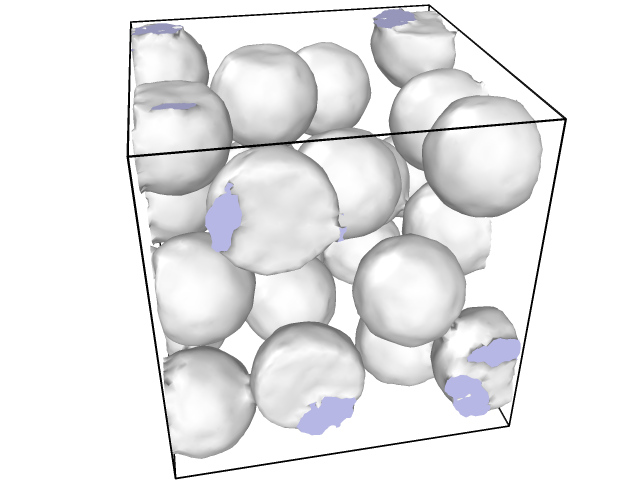
\includegraphics[width=10cm]{Cap_5/spheres.png}
  \caption[Nanopartículas esféricas de material para el sinterizado]{Imagen de las nanopartículas esféricas de material.}
  \label{C5:fg:sintInicial}
\end{figure}

El procedimiento para simular el sinterizado fue el siguiente:

\begin{itemize}
 \item Relajación de la muestra a volumen constante y temperatura constante de 650K (justo debajo de la temperatura
de transición vítrea) durante unos pocos ps.
 \item Aplicación de hasta 10 ps de presión compresiva (400 bar).
 \item Se repitieron los dos pasos anteriores hasta lograr las porosidades deseadas.
 \item Para finalizar, se realiza una nueva relajación de la muestra:
 \begin{itemize}
  \item Temple a temperatura cero mediante una velocidad de enfriamiento de $6.5 \cdot 10^{14} K/s$.
  \item Disminución de la presión a cero.
  \item Calentamiento a $6.5 \cdot 10^{14} K/s$ para llegar a la temperatura de simulación (300K).
  \item Reducción de la presión a cero, manteniendo la temperatura constante.
 \end{itemize}
\end{itemize}

Se prepararon muestras con distintas porosidades iniciales (3.3\%, 5.8\% y 13.1\%, véase Figuras~\ref{C5:fg:sint} y \ref{C5:fg:sint2}).
Estas muestras estabilizadas fueron luego utilizadas para realizar carga uniaxial de compresión y tracción. Todas las coordenadas atómicas fueron recalculadas a cada paso, en relación con la velocidad de deformación requerida, la cual fue de $10^9 /s$, valor apropiado para experimentos de choque compresivo.

\begin{figure}[h!]
  \centering
  \begin{tabular} {c}
     \subfloat[Porosidad 3.3\%]{
	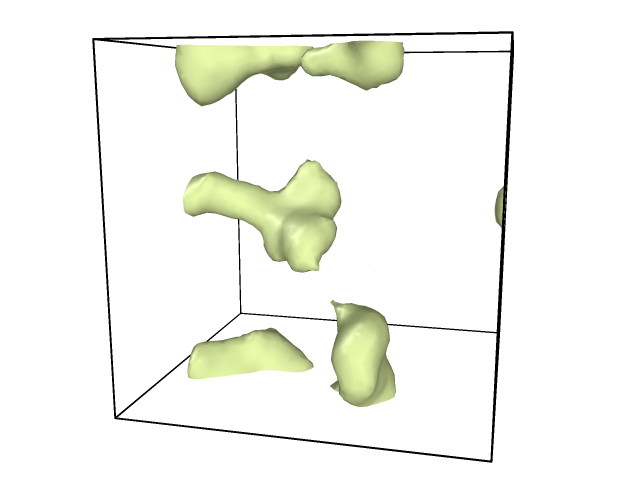
\includegraphics[width=8cm]{Cap_5/3_0strain.png}} \\
     \subfloat[Porosidad 5.8\%]{
	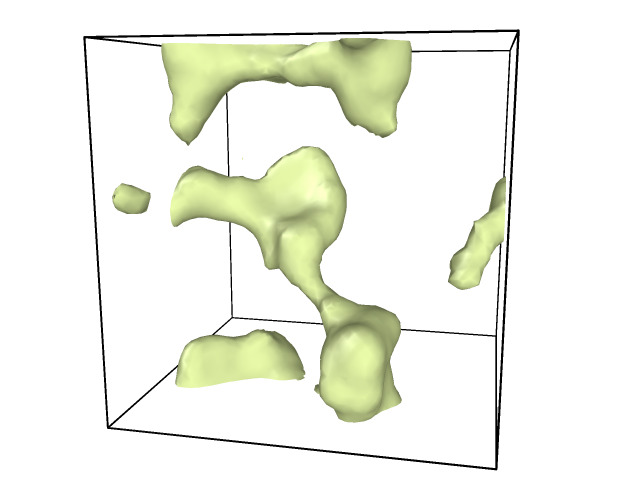
\includegraphics[width=8cm]{Cap_5/6_0strain.png}} \\
     \subfloat[Porosidad 13.1\%]{
	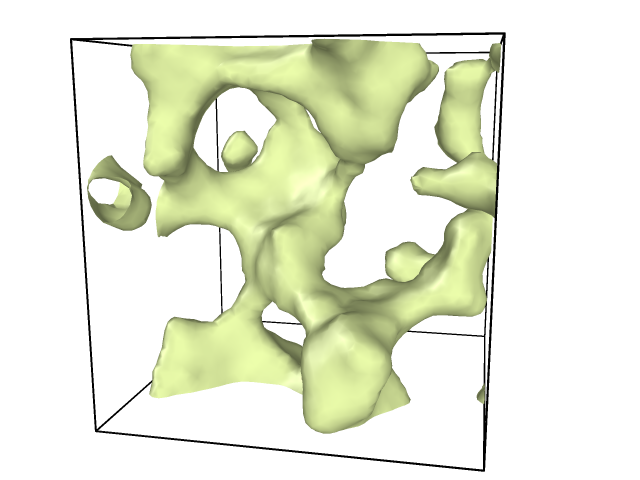
\includegraphics[width=8cm]{Cap_5/13_0strain_pores.png}}
  \end{tabular}
  \caption[Porosidad en las muestras sinterizadas]{Imágenes de la red de poros de la muestra sinterizada, para todas las porosidades realizadas.}
  \label{C5:fg:sint}
\end{figure}

\begin {figure}[h!]
 \centering
  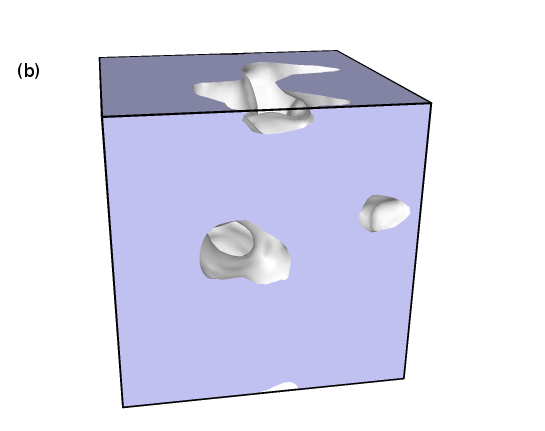
\includegraphics[width=8cm]{Cap_5/spheres3.png}
  \caption[Muestra sinterizada, porosidad 13.1\%]{Imagen de la muestra sinterizada, porosidad 13.1\%.}
  \label{C5:fg:sint2}
\end {figure}

%----------------------------------------------------------------------------------------
%	SECTION 3
%----------------------------------------------------------------------------------------

\section{Resultados}
\label{S5_4}

\subsection{Carga Uniaxial del BMG Poroso}

\cambioGrande{EN ESTA SECCION SE CAMBIO EL ORDEN GENERAL DE LOS PARRAFOS PARA TENER UN MEJOR ORDENAMIENTO DE FIGURAS. ADEMAS SE DESDOBLARON VARIAS IMAGENES}

A continuación presentamos resultados para deformación puramente uniaxial, la cual es adecuada para realizar comparaciones con resultados de experimentos a altas velocidades de deformación, donde las deformaciones laterales pueden ser despreciadas.

La \fref{C5:fg:svf} muestra la evolución de la densidad en las muestras porosas:
\begin{itemize}
 \item Para el caso de compresión, hemos agregado unas líneas a trazos que indican el valor de deformación ($\epsilon$) para el cual los poros se cierran completamente, es decir, cuando la fracción de volumen sólido es igual a 1. Para una porosidad de 3\% el valor de $\epsilon$ es de 0.05, para porosidad de 6\% $\epsilon = 0.065$ y para porosidad 13\%, $\epsilon = 0.12$. En algunas de las figuras de esta sección aparecerán estas líneas nuevamente, a fin de observar si este evento implica cambios en el comportamiento plástico.
 \item Para el caso de tracción, el uso de condiciones de borde periódicas evita que los poros se cierren incluso a altas deformaciones uniaxiales, dado que no hay deformaciones laterales.
\end{itemize}

\begin{figure}[h!]
  \centering
  \begin{tabular} {c}
     \subfloat[Compresión]{
	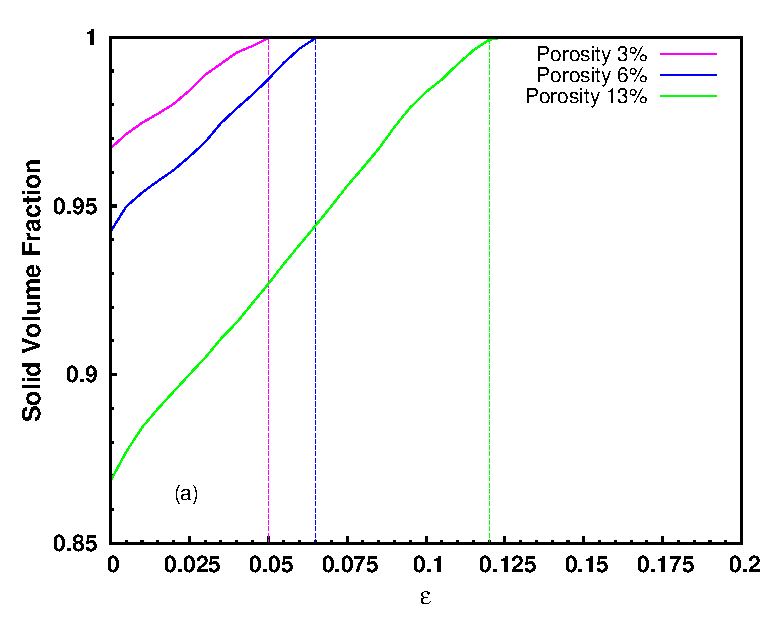
\includegraphics[width=8cm]{Cap_5/SVF_strain_comp_dash.eps}
	\label{C5:fg:svfComp}}
     \subfloat[Tracción]{
	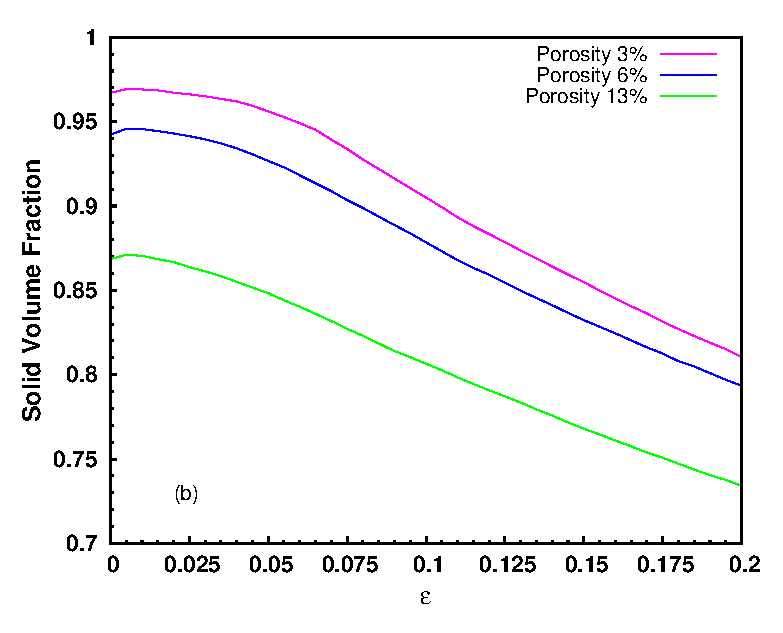
\includegraphics[width=8cm]{Cap_5/SVF_strain_tens.eps}
	\label{C5:fg:svfTens}}
  \end{tabular}
  \caption[Fracción de volumen sólido (SVF) versus deformación]{Fracción de volumen sólido (SVF) versus deformación. En (a), las líneas a trazos indican la deformación a la cual los poros se cierran por completo}
  \label{C5:fg:svf}
\end{figure}

%COMPRESION

La \fref{C5:fg:PzzComp} grafica la presión en el eje de carga versus deformación para esfuerzos de compresión. La \fref{C5:fg:stressComp},
a su vez, grafica la tensión de Von Mises versus deformación para esfuerzos de compresión.
Ambas gráficas nos indican que la presencia de porosidad promueve el inicio de la plasticidad. Los poros actúan como concentradores de tensión,
facilitando la aparición de STZs y bandas de corte. Esta plasticidad temprana comienza a
cerrar los poros, produciendo una curva donde la deformación $\epsilon$ aumenta mientras que la presión se mantiene baja.
Cuando los poros se cierran, la presión aumenta más aceleradamente, como puede apreciarse en la porción de la curva posterior
a la línea de trazos. Podemos también observar que el comportamiento de las muestras porosas luego de las líneas de trazos es
muy similar al comportamiento de la muestra sin porosidad, validando el hecho de que a ese punto ya no hay más porosidad (esto también puede observarse en la gráfica de temperatura versus deformación, \fref{C5:fg:tempComp}). Basándonos en la Figura, podemos concluir que a mayor porosidad, se necesita menor esfuerzo para cerrar los poros (denotado por la altura de las líneas a trazos), pero esto ocurre a mayores deformaciones.

\begin{figure}[H]
  \centering
%  \begin{tabular} {c}
%     \subfloat[Compresión]{
	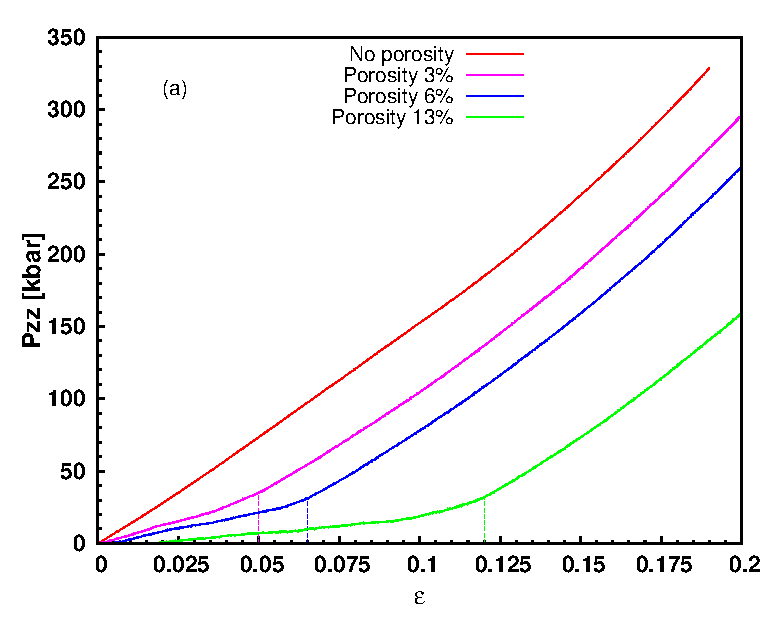
\includegraphics[width=8cm]{Cap_5/Pzz_strain_comp_dash.eps}
	\caption[Presión en el eje Z vs deformación para esfuerzos de compresión]{Presión en el eje Z vs deformación para esfuerzos de compresión.}
	\label{C5:fg:PzzComp}
%	\label{C5:fg:PzzComp}}
%     \subfloat[Tracción]{
%	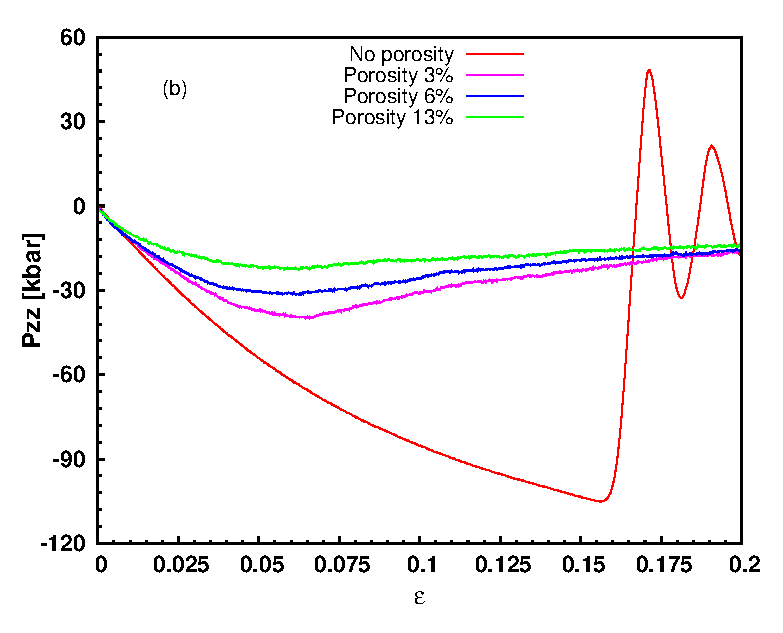
\includegraphics[width=8cm]{Cap_5/Pzz_strain_tens.eps}
%	\label{C5:fg:PzzTens}}
%  \end{tabular}
%  \caption[Presión en el eje Z vs deformación]{Presión en el eje Z vs deformación.}
%  \label{C5:fg:pzz2}
\end{figure}

\begin{figure}[H]
  \centering
%  \begin{tabular} {c}
 %    \subfloat[Compresión]{
	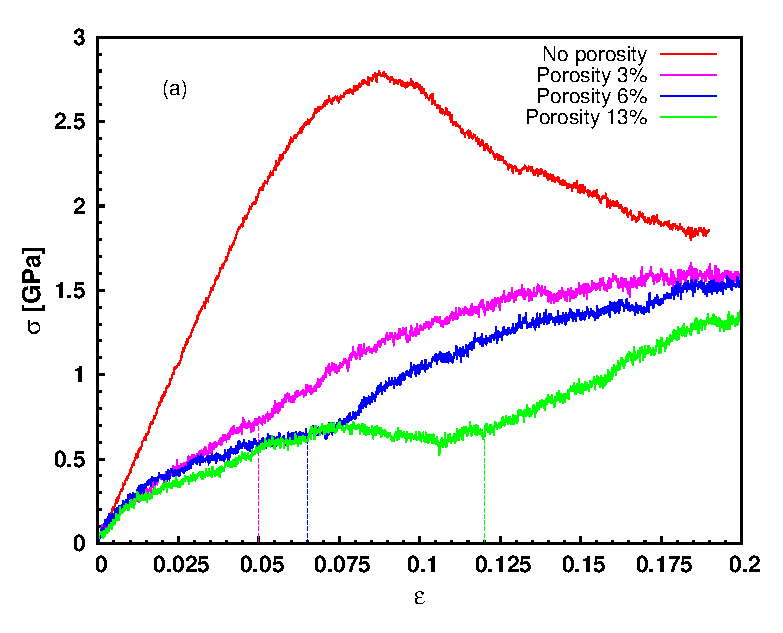
\includegraphics[width=8cm]{Cap_5/stress_strain_comp_dash.eps}
	\caption[Tensión de Von Mises vs deformación para esfuerzos de compresión]{Tensión de Von Mises vs deformación para esfuerzos de compresión.}
	\label{C5:fg:stressComp}
%	\label{C5:fg:stressComp}}
%     \subfloat[Tracción]{
%	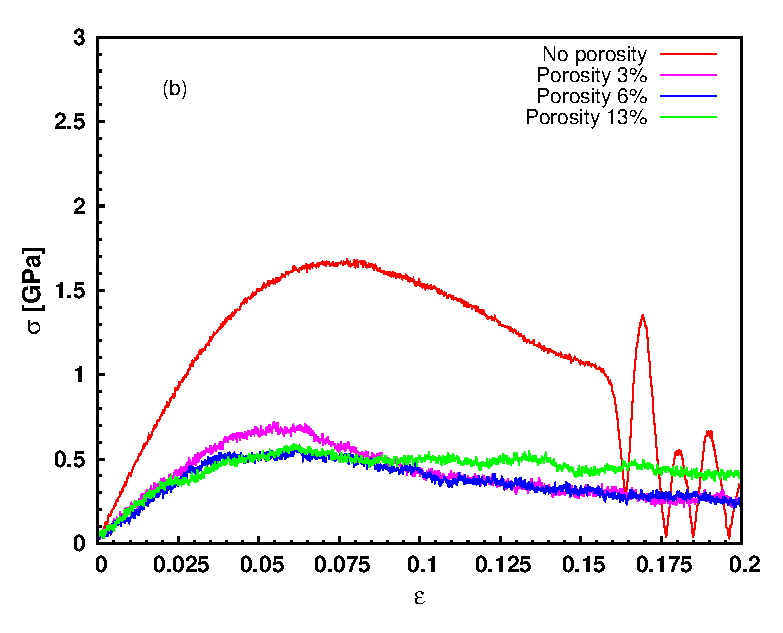
\includegraphics[width=8cm]{Cap_5/stress_strain_tens.eps}
%	\label{C5:fg:stressTens}}
%  \end{tabular}
%  \caption[Tensión de Von Mises vs deformación]{Tensión de Von Mises vs deformación.}
%  \label{C5:fg:stress}
\end{figure}

\begin{figure}[H]
  \centering
%  \begin{tabular} {c}
%     \subfloat[Compresión]{
	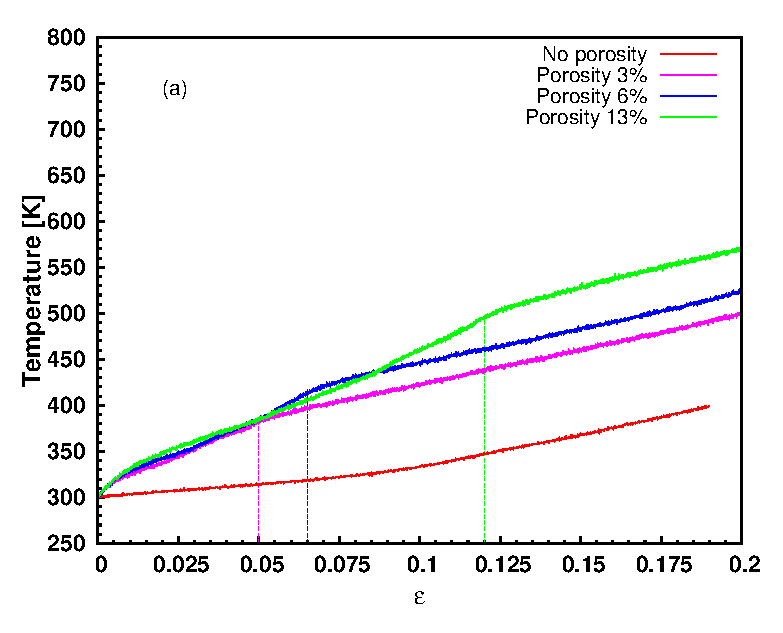
\includegraphics[width=8cm]{Cap_5/temp_strain_comp_dash.eps}
	\caption[Temperatura vs deformación para esfuerzos de compresión]{Temperatura vs deformación para esfuerzos de compresión.}
	\label{C5:fg:tempComp}
%	\label{C5:fg:tempComp}}
%     \subfloat[Tracción]{
%	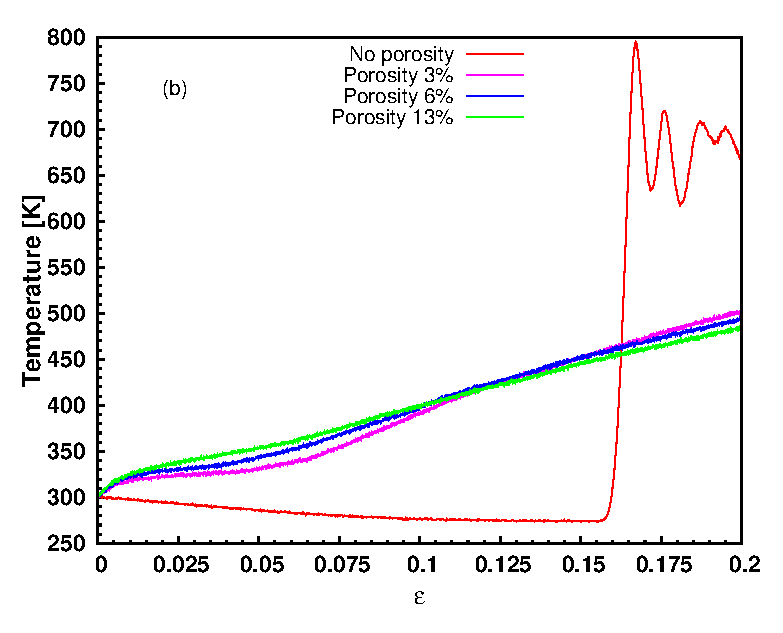
\includegraphics[width=8cm]{Cap_5/temp_strain_tens.eps}
%	\label{C5:fg:tempTens}}
%  \end{tabular}
%  \caption[Temperatura vs deformación]{Temperatura vs deformación.}
%  \label{C5:fg:temp}
\end{figure}

La \fref{C5:fg:tip3Comp} muestra curvas de poliedros de Voronoi versus deformación, para tensiones de compresión. El análisis por teselado de Voronoi es una técnica para caracterizar el ordenamiento local en vidrios metálicos amorfos, donde cada átomo es el centro de un poliedro de Voronoi,
completado por sus vecinos más cercanos. En \cite{arman10}, los átomos de tipo 3 son identificados como indicadores de plasticidad, por eso
son de gran importancia. La \fref{C5:fg:tip3Comp} muestra una caída en el número de los átomos tipo 3, la cual sucede luego de una fase prácticamente constante. Se ha pensado en este fenómeno como un indicador del inicio de la plasticidad \citep{arman10}. Sin embargo, nuestras curvas muestran un resultado contrario a la intuición, ya que la plasticidad comienza antes en las muestras con menor porosidad de acuerdo a nuestro análisis. Esto podría ser considerado como un indicador de que hay otros factores o procesos en juego que afectan los resultados.

\begin{figure}[H]
  \centering
%  \begin{tabular} {c}
%     \subfloat[Compresión]{
	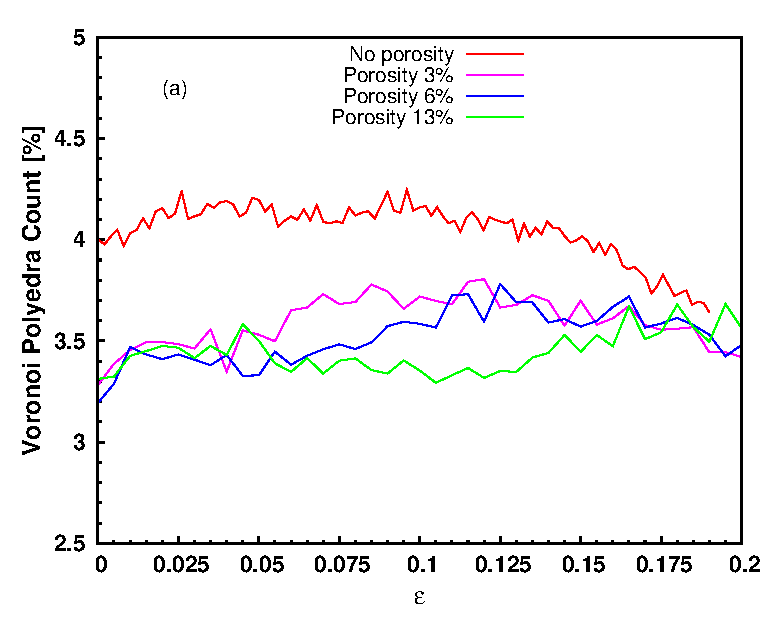
\includegraphics[width=8cm]{Cap_5/tipe3_strain_comp.eps}
	\caption[Poliedros de Voronoi tipo 3 vs deformación para esfuerzos de compresión]{Poliedros de Voronoi tipo 3 vs deformación para esfuerzos de compresión.}
	\label{C5:fg:tip3Comp}
%	\label{C5:fg:tip3Comp}}
%     \subfloat[Tracción]{
%	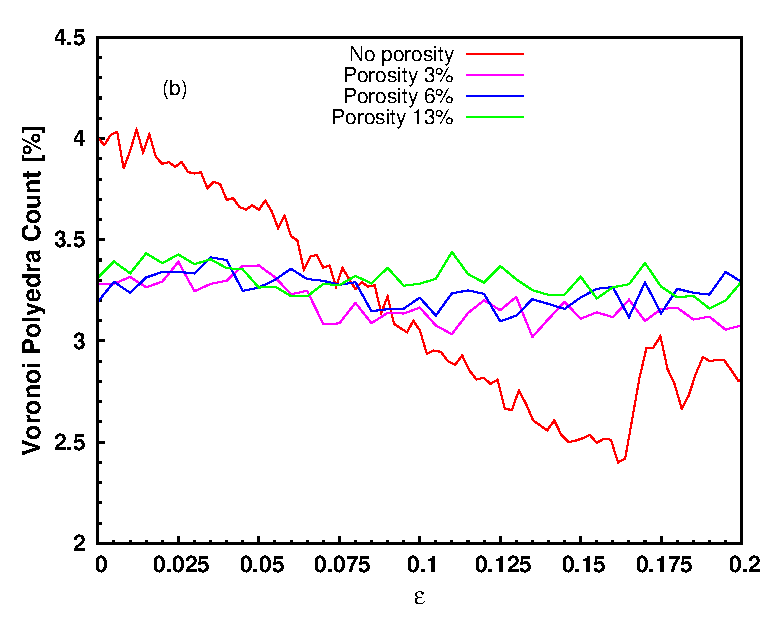
\includegraphics[width=8cm]{Cap_5/tipe3_strain_tens.eps}
%	\label{C5:fg:tip3Tens}}
%  \end{tabular}
%  \caption[Poliedros de Voronoi tipo 3 vs deformación]{Poliedros de Voronoi tipo 3 vs deformación.}
%  \label{C5:fg:tip3}
\end{figure}

Las Figuras~\ref{C5:fg:ss_comp_3}, \ref{C5:fg:ss_comp_6} y \ref{C5:fg:ss_comp_13} presentan la evolución de la deformación cortante en la muestra, para esfuerzos de compresión. Puede destacarse que los poros actúan como concentradores de tensiones, pero también representan un obstáculo para la propagación de bandas de corte \citep{wang10}. Las bandas de corte nuclean diagonalmente en el espacio entre poros, y la deformación atómica se acumula a lo largo de estas direcciones principales por el resto de la simulación, como puede observarse particularmente en la \fref{C5:fg:secuenciadef}. Un endurecimiento de la muestra ocurre algunos momentos previo al cierre total de los poros, tal y como ha apreciado \cite{yuan14} y puede verse en la \fref{C5:fg:PzzComp}.

\begin{figure}[H]
  \centering
  \begin{tabular}{c}
    \subfloat[Porosidad 3\%, sin deformación]{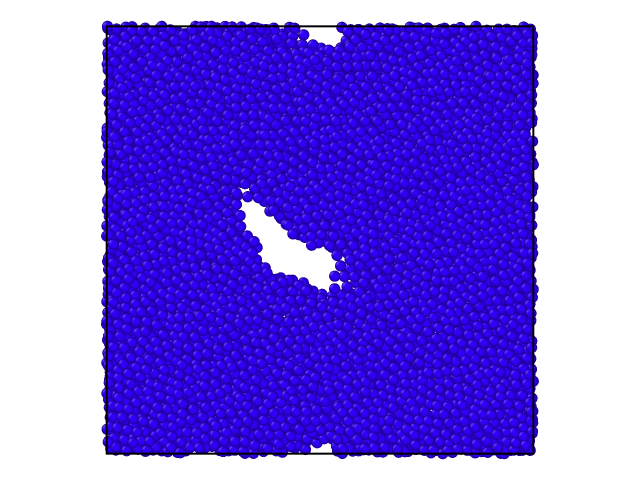
\includegraphics[width=8cm]{Cap_5/3_0strain_pores.png}} \\
    \subfloat[Porosidad 3\%, deformación 5\%]{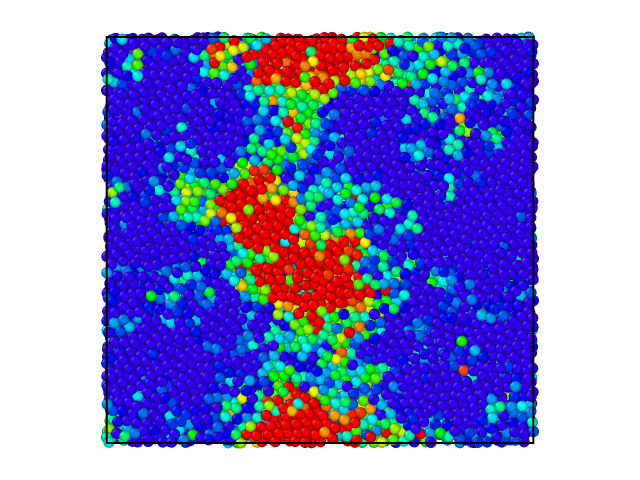
\includegraphics[width=8cm]{Cap_5/3_5strain_comp.png}}
    \subfloat[Porosidad 3\%, deformación 12\%]{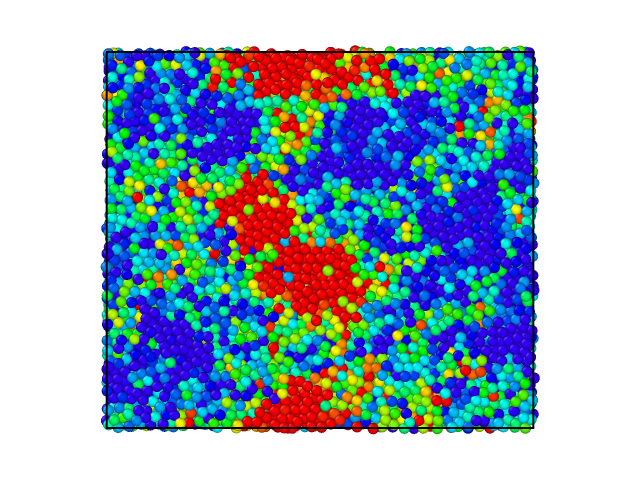
\includegraphics[width=8cm]{Cap_5/3_12strain_comp.png}}\\
    \\ 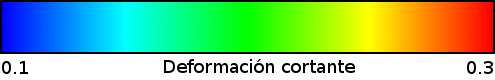
\includegraphics[width=6cm]{Cap_5/escala.png}
  \end{tabular}
  \caption[Sección de la muestra con porosidad 3\%, deformación por compresión]{Coloreado de una sección de la muestra con porosidad 3\% según la deformación cortante. (a) Estado inicial de la muestra (b) 5\% deformación por compresión (c) 12\% deformación por compresión.}
  \label{C5:fg:ss_comp_3}
\end{figure}

\begin{figure}[H]
  \centering
  \begin{tabular}{c}
    \subfloat[Porosidad 6\%, sin deformación]{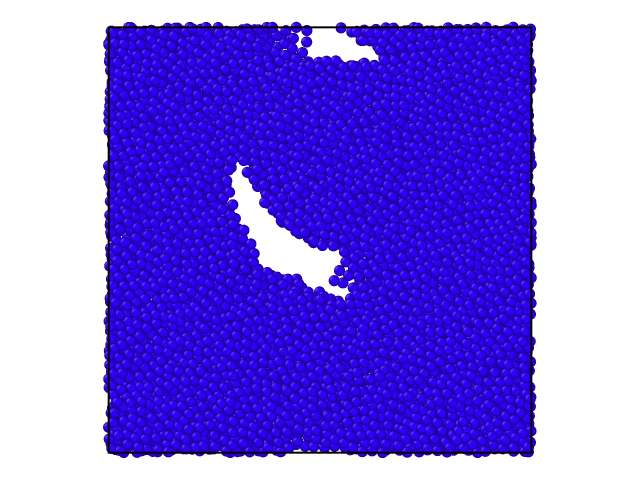
\includegraphics[width=8cm]{Cap_5/6_0strain_pores.png}} \\
    \subfloat[Porosidad 6\%, deformación 5\%]{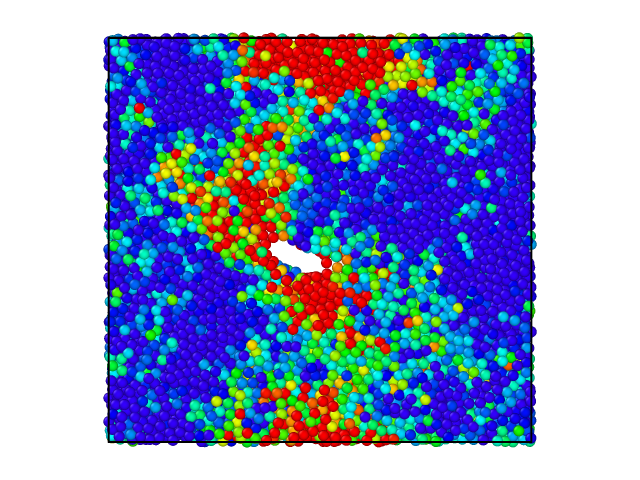
\includegraphics[width=8cm]{Cap_5/6_5strain_comp.png}}
    \subfloat[Porosidad 6\%, deformación 12\%]{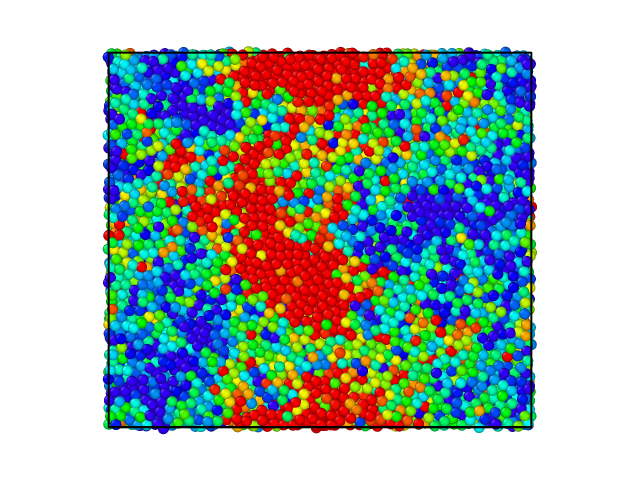
\includegraphics[width=8cm]{Cap_5/6_12strain_comp.png}}\\
    \\ 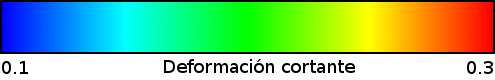
\includegraphics[width=6cm]{Cap_5/escala.png}
  \end{tabular}
  \caption[Sección de la muestra con porosidad 6\%, deformación por compresión]{Coloreado de una sección de la muestra con porosidad 6\% según la deformación cortante. (a) Estado inicial de la muestra (b) 5\% deformación por compresión (c) 12\% deformación por compresión.}
  \label{C5:fg:ss_comp_6}
\end{figure}

\begin{figure}[H]
  \centering
  \begin{tabular}{c}
    \subfloat[Porosidad 13\%, sin deformación]{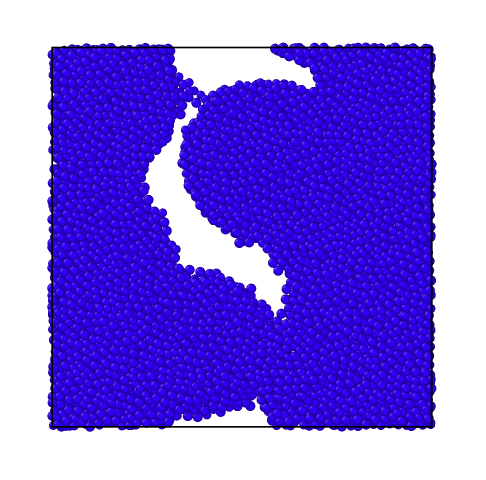
\includegraphics[width=7cm]{Cap_5/13_0strain.png}} \\
    \subfloat[Porosidad 13\%, deformación 5\%]{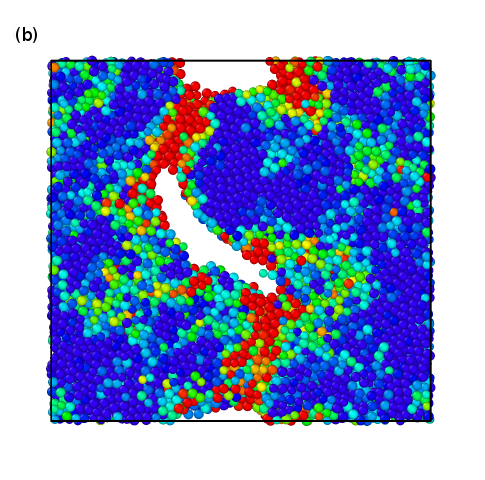
\includegraphics[width=7cm]{Cap_5/13_5strain_comp.png}}
    \subfloat[Porosidad 13\%, deformación 12\%]{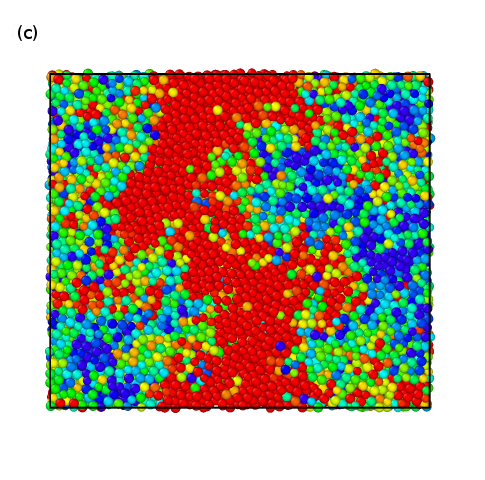
\includegraphics[width=7cm]{Cap_5/13_12strain_comp.png}}\\
    \\ 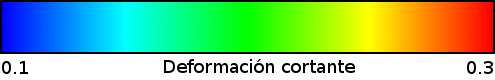
\includegraphics[width=6cm]{Cap_5/escala.png}
  \end{tabular}
  \caption[Sección de la muestra con porosidad 13\%, deformación por compresión]{Coloreado de una sección de la muestra con porosidad 13\% según la deformación cortante. (a) Estado inicial de la muestra (b) 5\% deformación por compresión (c) 12\% deformación por compresión.}
  \label{C5:fg:ss_comp_13}
\end{figure}

\begin{figure}[H]
  \centering
  \begin{tabular}{c}
    \subfloat[Porosidad 6\%, sin deformación]{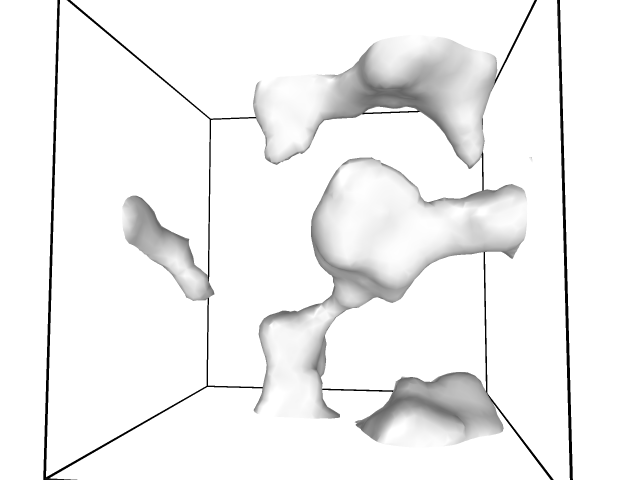
\includegraphics[width=8cm]{Cap_5/porosidad_6_shearstrain04_0.png}}
    \subfloat[Porosidad 6\%, deformación 5\%]{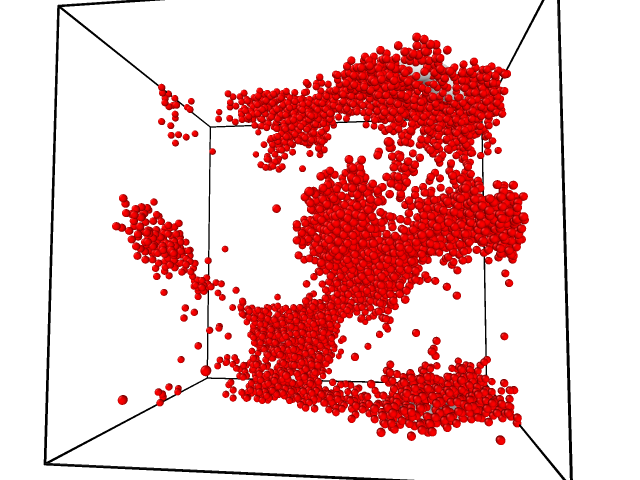
\includegraphics[width=8cm]{Cap_5/porosidad_6_shearstrain04_006.png}} \\
    \subfloat[Porosidad 6\%, deformación 12\%]{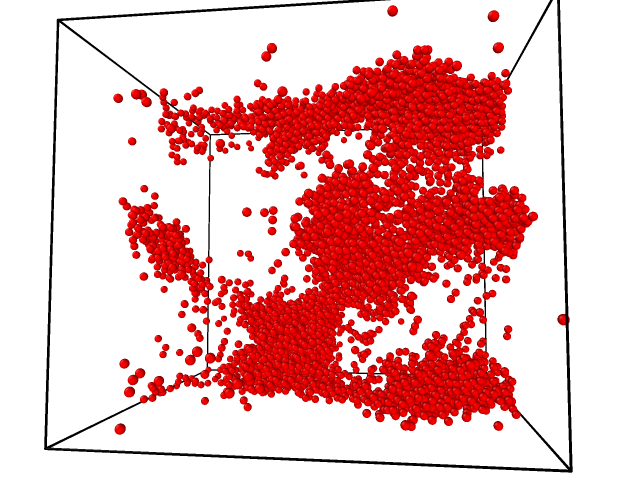
\includegraphics[width=8cm]{Cap_5/porosidad_6_shearstrain04_012.png}}
    \subfloat[Porosidad 6\%, deformación 12\%]{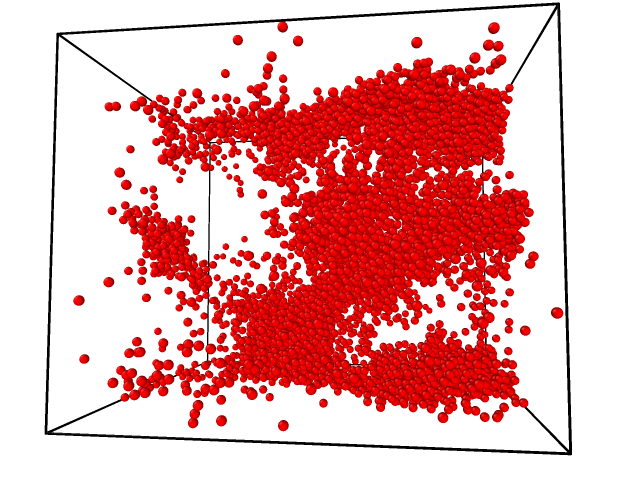
\includegraphics[width=8cm]{Cap_5/porosidad_6_shearstrain04_018.png}}
  \end{tabular}
  \caption[Selección de átomos con deformación cortante elevada en la muestra con porosidad 6\%, deformación por compresión]{Selección de átomos con deformación cortante superior a 0.4 en la muestra con porosidad 6\%. Todos los átomos en rojo cumplen dicha condición. (a) Estado inicial de la muestra. (b) 6\% deformación por compresión. (c) 12\% deformación por compresión. (d) 18\% deformación por compresión.}
  \label{C5:fg:secuenciadef}
\end{figure}

%TRACCION

En tracción las muestras se comportan en forma diferente. Como ya se ha dicho los poros no se cierran en tracción, como sí lo hacían en compresión.
Las Figuras~\ref{C5:fg:PzzTens} y \ref{C5:fg:stressTens} muestran, particularmente a 13\% de porosidad,
pero similarmente a otras porosidades, que luego de un cierto punto la deformación aumenta mientras la presión se mantiene constante o
incluso disminuye. Mediante el análisis de algunas imágenes de la muestra, como las que aparecen en las Figuras~\ref{C5:fg:ss_tens_3}, \ref{C5:fg:ss_tens_6} o \ref{C5:fg:ss_tens_13}, observamos que los poros crecen a una velocidad aproximadamente constante a medida que la deformación de la muestra aumenta. En dichas Figuras se presenta la muestra coloreada con la deformación cortante.

\begin{figure}[H]
  \centering
%  \begin{tabular} {c}
%     \subfloat[Compresión]{
%	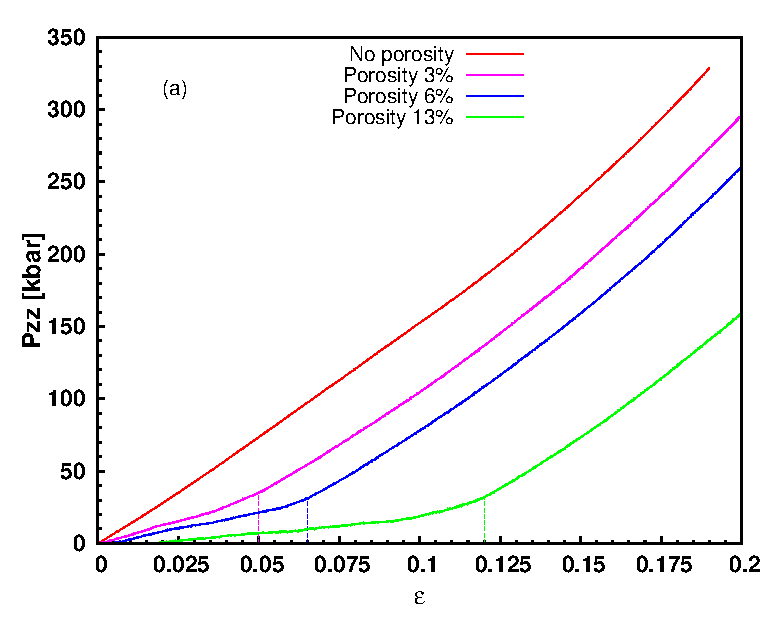
\includegraphics[width=8cm]{Cap_5/Pzz_strain_comp_dash.eps}
%	\label{C5:fg:PzzComp}}
%     \subfloat[Tracción]{
	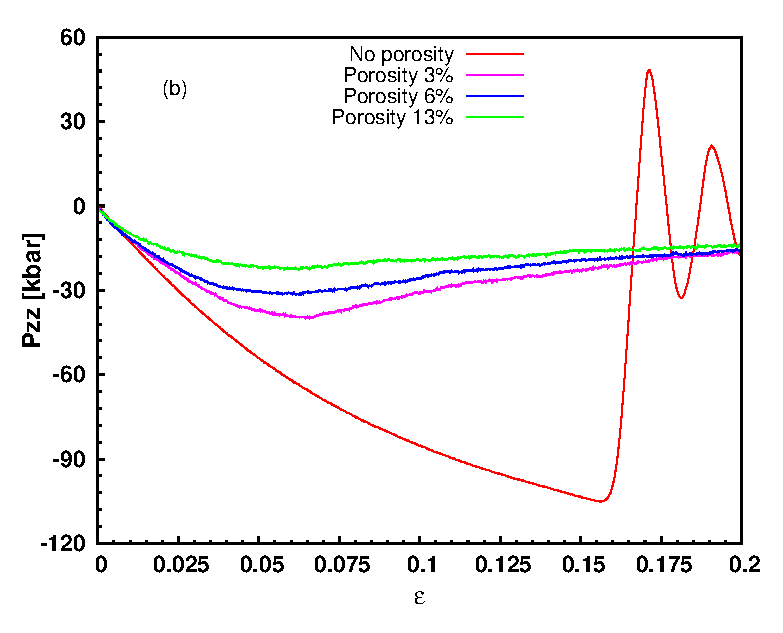
\includegraphics[width=8cm]{Cap_5/Pzz_strain_tens.eps}
	\caption[Presión en el eje Z vs deformación para esfuerzos de tracción]{Presión en el eje Z vs deformación para esfuerzos de tracción.}
	\label{C5:fg:PzzTens}
%	\label{C5:fg:PzzTens}}
%  \end{tabular}
%  \caption[Presión en el eje Z vs deformación]{Presión en el eje Z vs deformación.}
%  \label{C5:fg:pzz2}
\end{figure}

\begin{figure}[H]
  \centering
%  \begin{tabular} {c}
%     \subfloat[Compresión]{
%	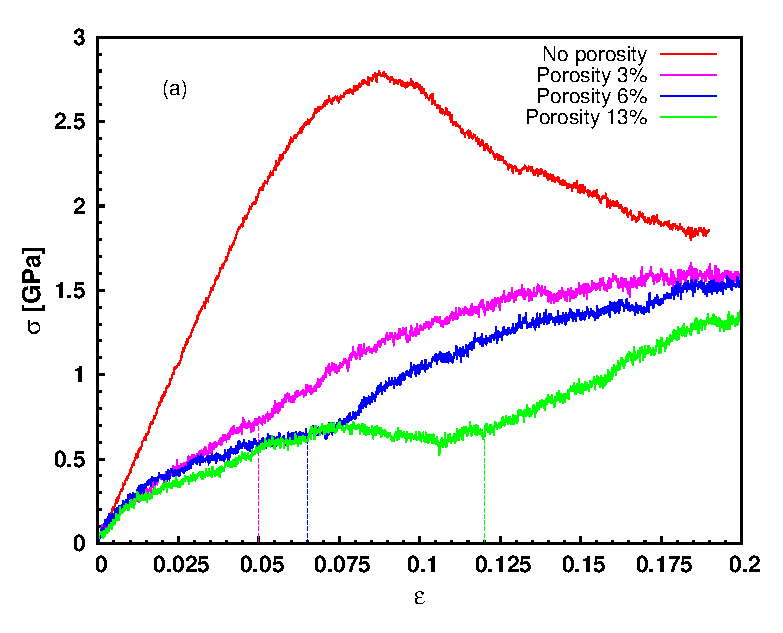
\includegraphics[width=8cm]{Cap_5/stress_strain_comp_dash.eps}
%	\label{C5:fg:stressComp}}
%     \subfloat[Tracción]{
	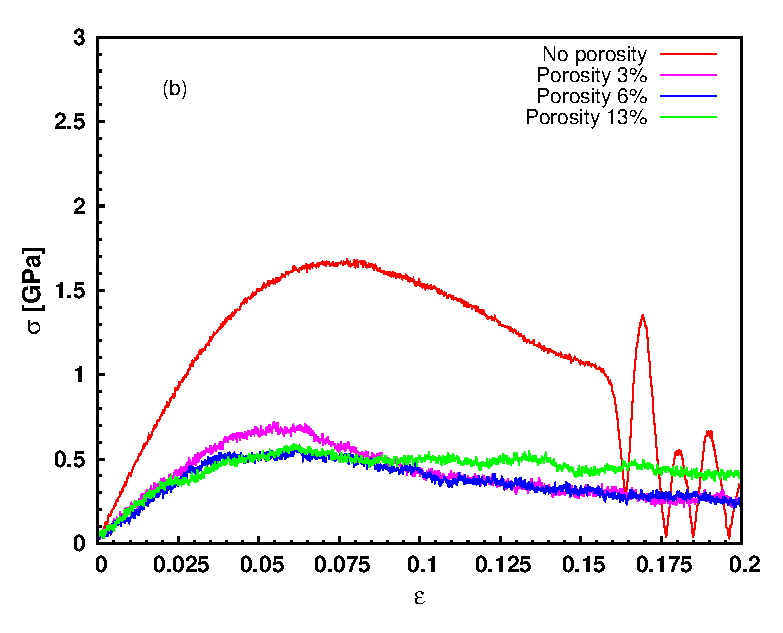
\includegraphics[width=8cm]{Cap_5/stress_strain_tens.eps}
	\caption[Tensión de Von Mises vs deformación para esfuerzos de tracción]{Tensión de Von Mises vs deformación para esfuerzos de tracción.}
	\label{C5:fg:stressTens}
%	\label{C5:fg:stressTens}}
%  \end{tabular}
%  \caption[Tensión de Von Mises vs deformación]{Tensión de Von Mises vs deformación.}
  \label{C5:fg:stress}
\end{figure}

La \fref{C5:fg:tip3Tens} muestra las curvas de poliedros de Voronoi para tensiones de tracción. En esta gráfica, los átomos de tipo 3
prácticamente no varían en las muestras con porosidad, lo que implicaría que no hay formación de STZs. Para la muestra no porosa, el número de átomos tipo 3 se vuelve aproximadamente constante luego de que se ha nucleado el poro. Esto conduce a pensar que, dada las condiciones de las muestras, se facilita el movimiento de los átomos alrededor de los poros, lo cual evita la formación de STZs fuera de los alrededores de los poros. Para apoyar esta idea, las Figuras~\ref{C5:fg:ss_tens_3}, \ref{C5:fg:ss_tens_6} y \ref{C5:fg:ss_tens_13} nos muestran que la deformación cortante se concentra principalmente alrededor de los poros. Debe ser mencionado que la posición relativa entre átomos que se encuentran lejanos de los poros se mantiene aproximadamente igual.

\begin{figure}[H]
  \centering
  \begin{tabular}{c}
    \subfloat[Porosidad 3\%, sin deformación]{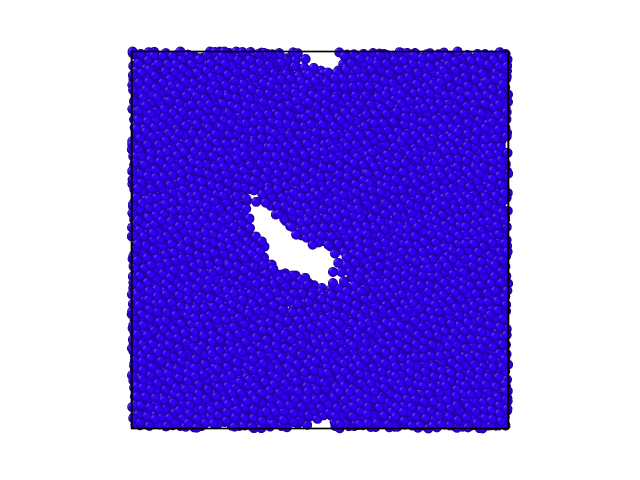
\includegraphics[width=8cm]{Cap_5/3_0strain_pores_tens.png}}
    \subfloat[Porosidad 3\%, deformación 5\%]{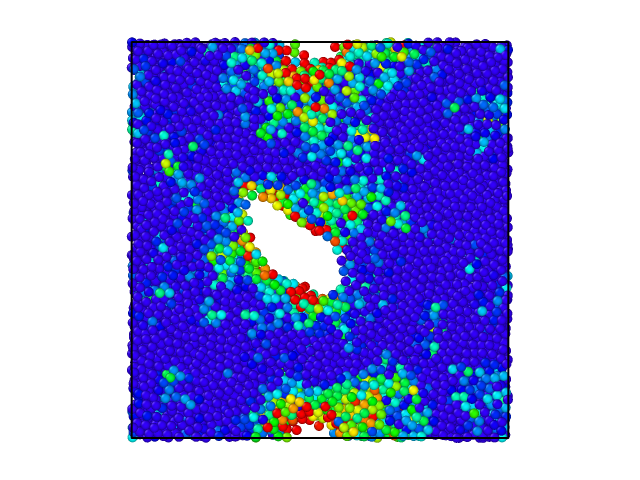
\includegraphics[width=8cm]{Cap_5/3_5strain_tens.png}} \\
    \subfloat[Porosidad 3\%, deformación 12\%]{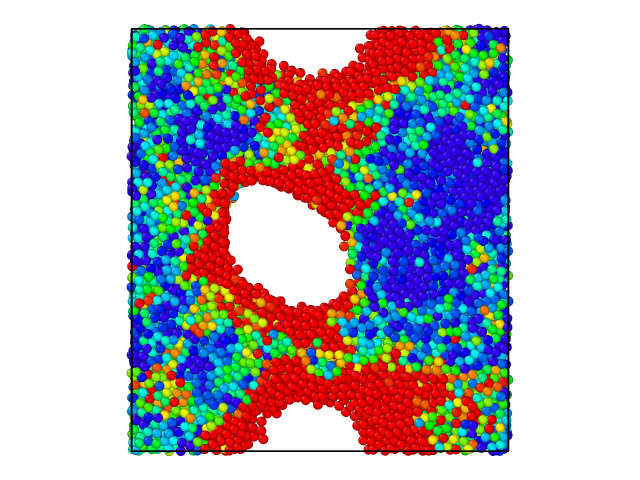
\includegraphics[width=8cm]{Cap_5/3_12strain_tens.png}}
    \subfloat[Porosidad 3\%, deformación 20\%]{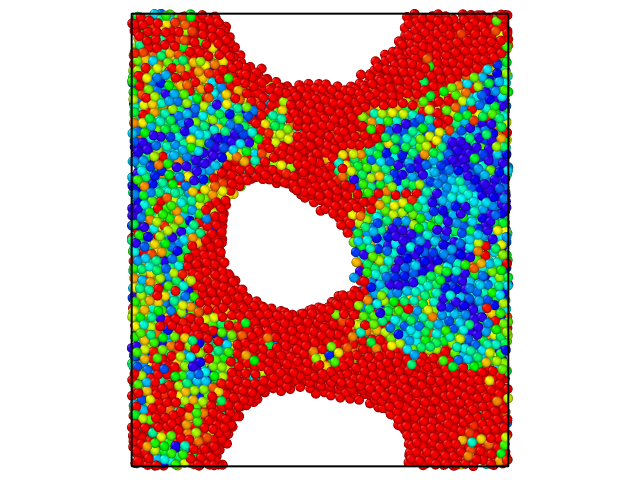
\includegraphics[width=8cm]{Cap_5/3_20strain_tens.png}}\\
    \\ 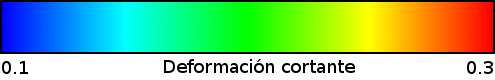
\includegraphics[width=6cm]{Cap_5/escala.png}
  \end{tabular}
  \caption[Sección de la muestra con porosidad 3\%, deformación por tracción]{Coloreado de una sección de la muestra con porosidad 3\% según la deformación cortante. (a) Estado inicial de la muestra. (b) 5\% deformación por tracción (c) 12\% deformación por tracción. (d) 20\% deformación por tracción.}
  \label{C5:fg:ss_tens_3}
\end{figure}

\begin{figure}[H]
  \centering
  \begin{tabular}{c}
    \subfloat[Porosidad 6\%, sin deformación]{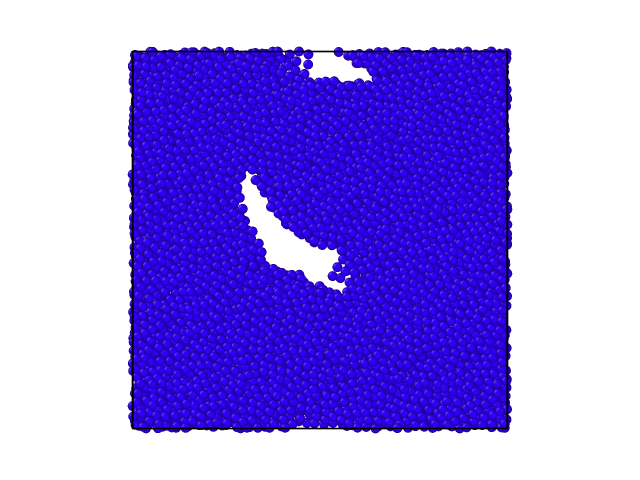
\includegraphics[width=8cm]{Cap_5/6_0strain_pores_tens.png}} 
    \subfloat[Porosidad 6\%, deformación 5\%]{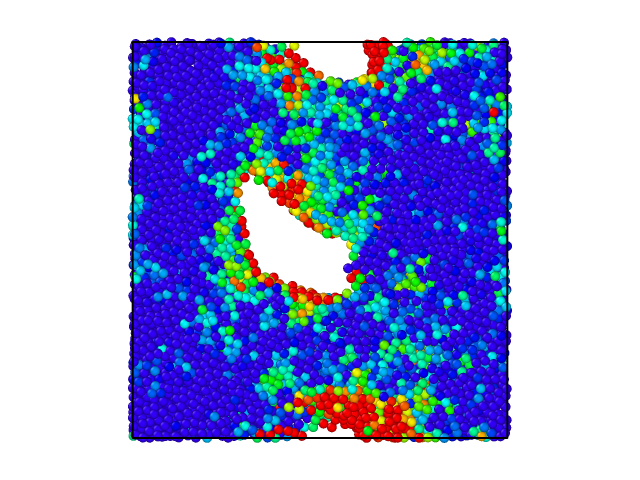
\includegraphics[width=8cm]{Cap_5/6_5strain_tens.png}} \\
    \subfloat[Porosidad 6\%, deformación 12\%]{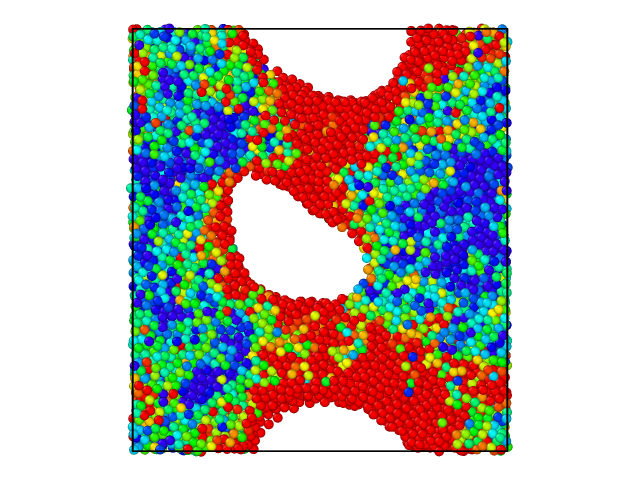
\includegraphics[width=8cm]{Cap_5/6_12strain_tens.png}}
    \subfloat[Porosidad 6\%, deformación 20\%]{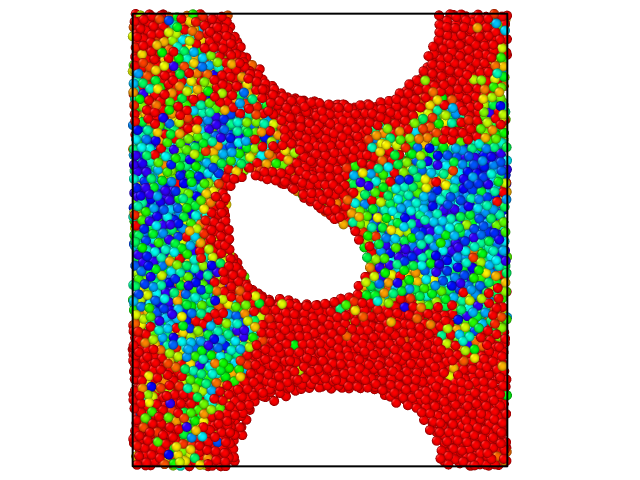
\includegraphics[width=8cm]{Cap_5/6_20strain_tens.png}}\\
    \\ 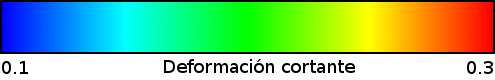
\includegraphics[width=6cm]{Cap_5/escala.png}
  \end{tabular}
  \caption[Sección de la muestra con porosidad 6\%, deformación por tracción]{Coloreado de una sección de la muestra con porosidad 6\% según la deformación cortante. (a) Estado inicial de la muestra. (b) 5\% deformación por tracción (c) 12\% deformación por tracción. (d) 20\% deformación por tracción.}
  \label{C5:fg:ss_tens_6}
\end{figure}


\begin{figure}[H]
  \centering
  \begin{tabular}{c}
    \subfloat[Porosidad 13\%, sin deformación]{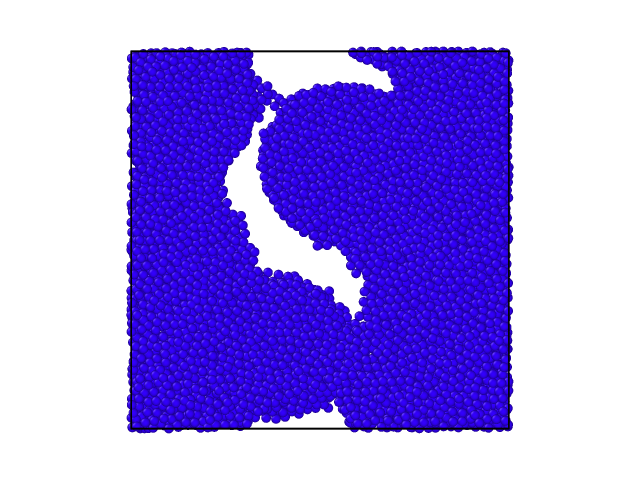
\includegraphics[width=8cm]{Cap_5/13_0strain_pores_tens.png}} 
    \subfloat[Porosidad 13\%, deformación 5\%]{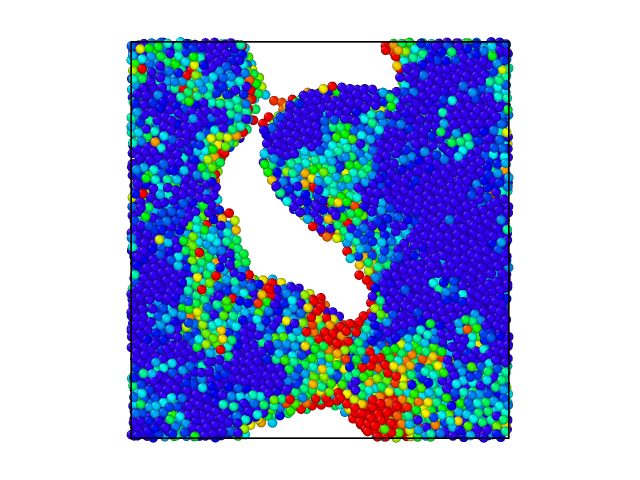
\includegraphics[width=8cm]{Cap_5/13_5strain_tens.png}}\\
    \subfloat[Porosidad 13\%, deformación 12\%]{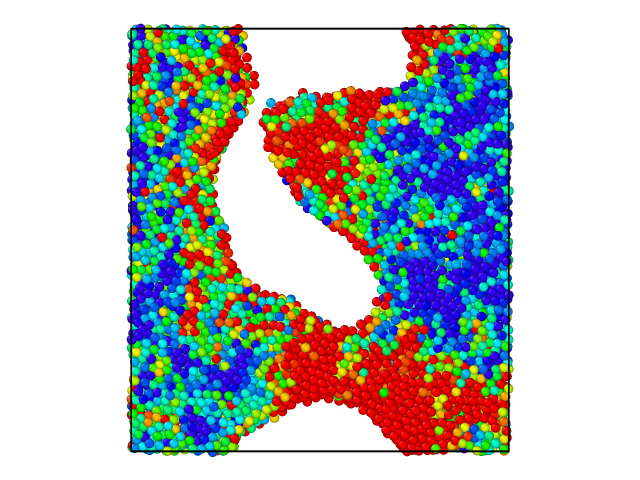
\includegraphics[width=8cm]{Cap_5/13_12strain_tens.png}}
    \subfloat[Porosidad 13\%, deformación 20\%]{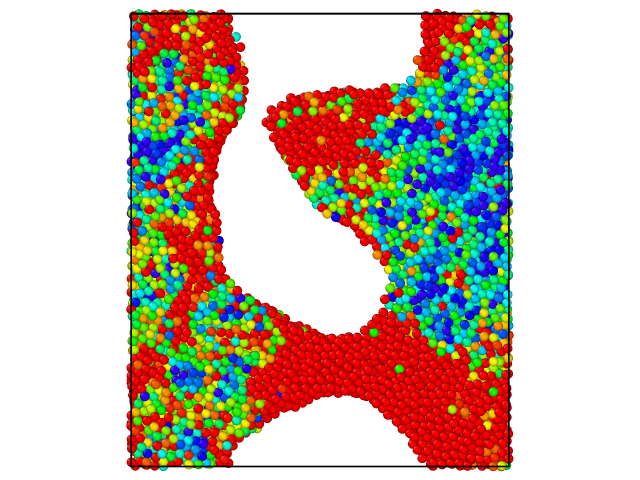
\includegraphics[width=8cm]{Cap_5/13_20strain_tens2.png}}\\
    \\ \includegraphics[width=6cm]{Cap_5/escala.png}
  \end{tabular}
  \caption[Sección de la muestra con porosidad 13\%, deformación por tracción]{Coloreado de una sección de la muestra con porosidad 13\% según la deformación cortante. (a) Estado inicial de la muestra. (b) 5\% deformación por tracción (c) 12\% deformación por tracción. (d) 20\% deformación por tracción.}
  \label{C5:fg:ss_tens_13}
\end{figure}

\begin{figure}[H]
  \centering
%  \begin{tabular} {c}
%     \subfloat[Compresión]{
%	\includegraphics[width=8cm]{Cap_5/tipe3_strain_comp.eps}
%	\label{C5:fg:tip3Comp}}
%     \subfloat[Tracción]{
	\includegraphics[width=8cm]{Cap_5/tipe3_strain_tens.eps}
	\caption[Poliedros de Voronoi tipo 3 vs deformación para esfuerzos de tracción]{Poliedros de Voronoi tipo 3 vs deformación para esfuerzos de tracción.}
	\label{C5:fg:tip3Tens}
%	\label{C5:fg:tip3Tens}}
%  \end{tabular}
%  \caption[Poliedros de Voronoi tipo 3 vs deformación]{Poliedros de Voronoi tipo 3 vs deformación.}
%  \label{C5:fg:tip3}
\end{figure}

\FloatBarrier

\subsection{Influencia de la velocidad de enfriamiento}
\label{C5:relaj}

En la \sref{S5_3}, se detalló el proceso utilizado para realizar el sinterizado de la muestra. Las velocidades utilizadas para el enfriamiento/calentamiento durante el proceso final de relajación de la muestra fueron de $6.5 \cdot 10^{14} K/s$. Inicialmente, se utilizó esta velocidad alta debido a las limitaciones computacionales. Sin embargo, finalmente también se pudo probar con una velocidad menor, más cercana a la velocidad de enfriamiento con la que fue creada la muestra de cobre-circonio original: $6.5 \cdot 10^{12} K/s$. La elección de esta velocidad no fue azarosa: debía disminuir lo suficiente con respecto a la velocidad anterior como para poder observar cambios en el comportamiento elastoplástico de la muestra, pero no demasiado como para permitir la cristalización del material.

Lo primero que debe ser considerado es que si se interrumpen las iteraciones de calentamiento-presión en un punto determinado y luego se realizan dos relajaciones distintas con las dos velocidades previamente mencionadas, las porosidades finales serán distintas. De hecho, la muestra que con una velocidad de $6.5 \cdot 10^{14} K/s$ tenía 3\% de porosidad, con $6.5 \cdot 10^{12} K/s$ no posee porosidad. Por esta razón, esta muestra se excluye en la presente sección. En la \tref{C5:tbl:porosityChange} se indican las porosidades resultantes para las dos velocidades de calentamiento/enfriamiento.

\begin{table}[htp]
\begin{center}
\begin{tabular}{c C{5cm} C{5cm}}
\hline
\textbf{Extracción de muestras} & \textbf{Porosidad para velocidad $6.5 \cdot 10^{14} K/s$} & \textbf{Porosidad para velocidad $6.5 \cdot 10^{12} K/s$} \\ \hline
\hline
Primera extracción & 13.1\% & 13.5\% \\ \hline
Segunda extracción & 5.8\% & 4.5\% \\ \hline
Tercer extracción & 3.3\% & 0\% \\ \hline
\end{tabular}
\end{center}
\caption[Porosidades resultantes a dos velocidades de calentamiento/enfriamiento distintas]{Porosidades resultantes a dos velocidades de calentamiento/enfriamiento distintas.}
\label{C5:tbl:porosityChange}
\end{table}

\cambio{En las Figuras {\ref{C5:fg:vel12_strain0_6}} y {\ref{C5:fg:vel12_strain0_13}} se muestran, a modo de comparación, muestras de porosidad similar generadas con las dos velocidades de enfriamiento/calentamiento estudiadas.} Del análisis de dichas Figuras, y de la \tref{C5:tbl:porosityChange}, concluimos que el cambio de velocidad no influye tanto en la porosidad final, sino más bien en la forma final de los poros en la muestra. Una menor velocidad implica que se requiere un tiempo mayor para lograr los cambios de temperatura deseados. Este tiempo adicional favorece el movimiento atómico y la difusión, resultando en disposiciones de menor energía. Esto puede observarse en las imágenes: para menores velocidades, el volumen de poros se concentra en un único poro que tiende a ser esférico, lo cual implica que hay menor superficie poro-material.

\begin {figure}[H]
 \centering
 \begin{tabular}{c c}
  \subfloat[Velocidad $6.5 \cdot 10^{14} K/s$]{\includegraphics[width=8cm]{Cap_5/porosidad6_vel14_strain0.png}} &
  \subfloat[Velocidad $6.5 \cdot 10^{12} K/s$]{\includegraphics[width=8cm]{Cap_5/porosidad6_vel12_strain0.png}}
 \end{tabular}
  \caption[Comparación de muestras con velocidades de enfriamiento/calentamiento distintas (porosidad 6\%)]{Estado inicial de las muestras generadas con velocidades de enfriamiento/calentamiento diferentes, para el caso de porosidad 6\%.}
  \label{C5:fg:vel12_strain0_6}
\end {figure}

\begin {figure}[H]
 \centering
  \begin{tabular}{c c}
  \subfloat[Velocidad $6.5 \cdot 10^{14} K/s$]{\includegraphics[width=8cm]{Cap_5/porosidad13_vel14_strain0.png}} &
  \subfloat[Velocidad $6.5 \cdot 10^{12} K/s$]{\includegraphics[width=8cm]{Cap_5/porosidad13_vel12_strain0.png}}
 \end{tabular}
  \caption[Comparación de muestras con velocidades de enfriamiento/calentamiento distintas (porosidad 13\%)]{Estado inicial de las muestras generadas con velocidades de enfriamiento/calentamiento diferentes, para el caso de porosidad 13\%.}
  \label{C5:fg:vel12_strain0_13}
\end {figure}

Las Figuras \ref{C5:fg:sint2_SVF}, \ref{C5:fg:sint2_PZZ} y \ref{C5:fg:sint2_VM} muestran, respectivamente, fracción de volumen sólido, presión en el eje de carga y tensión de Von Mises versus deformación, para las dos velocidades estudiadas y para los dos estados de carga analizados. Existe un aumento en la tensión máxima soportada y en el módulo de elasticidad, este último muy evidente en la \fref{C5:fg:sint2_VM}. Este cambio de propiedades puede deberse a una disminución de sitios concentradores de tensiones. Sin embargo, para grandes deformaciones (superiores a 7.5\$) los comportamientos son bastante similares en ambas velocidades, lo cual hace pensar que el comportamiento mecánico en esta etapa es más dependiente de la fracción de volumen sólido que de los parámetros del sinterizado.

\begin {figure}[H]
 \centering
   \begin{tabular}{c c}
  \subfloat[Compresión]{\includegraphics[width=8cm]{Cap_5/porosity_SVF_strain_vel12.eps}} &
  \subfloat[Tracción]{\includegraphics[width=8cm]{Cap_5/porosity_SVF_strain_vel12_trac.eps}}
   \end{tabular}
  \caption[SVF vs. deformación, velocidades $10^{12} K/s$ y $10^{14} K/s$]{Fracción de volumen sólido vs deformación. Velocidad de enfriamiento/calentamiento de $6.5 \cdot 10^{12} K/s$}
  \label{C5:fg:sint2_SVF}
\end {figure}

\begin {figure}[H]
 \centering
   \begin{tabular}{c c}
 \subfloat[Compresión]{\includegraphics[width=8cm]{Cap_5/porosity_PZZ_strain_comp_vel12.eps}} &
  \subfloat[Tracción]{\includegraphics[width=8cm]{Cap_5/porosity_PZZ_strain_trac_vel12.eps}}
   \end{tabular}
  \caption[Presión en eje de carga vs deformación, velocidades $10^{12} K/s$ y $10^{14} K/s$]{Presión en eje de carga vs deformación. Velocidad de enfriamiento/calentamiento de $6.5 \cdot 10^{12} K/s$}
  \label{C5:fg:sint2_PZZ}
\end {figure}

\begin {figure}[H]
 \centering
   \begin{tabular}{c c}
 \subfloat[Compresión]{\includegraphics[width=8cm]{Cap_5/porosity_VM_strain_comp_vel12.eps}} &
  \subfloat[Tracción]{\includegraphics[width=8cm]{Cap_5/porosity_VM_strain_trac_vel12.eps}}
   \end{tabular}
  \caption[Tensión de Von Mises vs deformación, velocidades $10^{12} K/s$ y $10^{14} K/s$]{Tensión de Von Mises vs deformación. Velocidad de enfriamiento/calentamiento de $6.5 \cdot 10^{12} K/s$}
  \label{C5:fg:sint2_VM}
\end{figure}

\FloatBarrier

\subsection{Influencia de la ubicación de los poros}

\cambioGrande{Imagenes nuevas}

Otro de los cambios que se plantearon en el proceso de sinterizado fue la ubicación de las partículas. Si bien los puntos que hicieron de centros de las partículas fueron escogidos al azar, dotando de generalidad a los resultados, las muestras de distintas porosidades fueron obtenidas a partir de la misma disposición de partículas. Simplemente se permitió realizar más iteraciones de calentamiento-presión para obtener las muestras de menor porosidad. Por ello en este apartado se estudia la influencia de la ubicación de los poros en los resultados obtenidos. Las Figuras \ref{C5:fg:comparativa6} y \ref{C5:fg:comparativa13} muestran, a modo comparativo, las muestras generadas con distintos patrones de porosidad.

\begin {figure}[H]
 \centering
 \begin{tabular}{c c}
  \subfloat[Primer sinterizado]{\includegraphics[width=8cm]{Cap_5/PrimerSintering_6_0strain.png}} &
  \subfloat[Segundo sinterizado]{\includegraphics[width=8cm]{Cap_5/SegundoSintering_6_0strain.png}}
 \end{tabular}
  \caption[Comparación de muestras con distinta distribución de poros (porosidad 6\%)]{Estado inicial de las muestras generadas con distinta distribución de poros, para el caso de porosidad 6\%.}
  \label{C5:fg:comparativa6}
\end {figure}

\begin {figure}[H]
 \centering
  \begin{tabular}{c c}
  \subfloat[Primer sinterizado]{\includegraphics[width=8cm]{Cap_5/PrimerSintering_13_0strain.png}} &
  \subfloat[Segundo sinterizado]{\includegraphics[width=8cm]{Cap_5/SegundoSintering_13_0strain.png}}
 \end{tabular}
  \caption[Comparación de muestras con distinta distribución de poros (porosidad 13\%)]{Estado inicial de las muestras generadas con distinta distribución de poros, para el caso de porosidad 13\%.}
  \label{C5:fg:comparativa13}
\end {figure}

\cambioGrande{ESTE PARRAFO: }Las Figuras \ref{C5:fg:2sint_SVF}, \ref{C5:fg:2sint_PZZ} y \ref{C5:fg:2sint_VM} muestran, respectivamente, fracción de volumen sólido, presión en el eje de carga y tensión de Von Mises versus deformación, para los dos sinterizados realizados. Se observa que el comportamiento es similar a lo largo de toda la simulación, a diferencia de lo que ocurría con las muestras a distintas velocidades de enfriamiento/calentamiento del apartado anterior (\ref{C5:relaj}). Las variaciones mínimas de las curvas son producto de las diferencias de porosidad inicial. Estos resultados dan la idea de que el comportamiento mecánico es más dependiente de la fracción de volumen sólido que de la forma de los poros, siempre y cuando los poros adopten una forma azarosa y repartida en el volumen de la muestra.

\begin {figure}[h!]
 \centering
   \begin{tabular}{c c}
  \subfloat[Compresión]{\includegraphics[width=8cm]{Cap_5/porosity_2sintering_SVF_comp.eps}} &
  \subfloat[Tracción]{\includegraphics[width=8cm]{Cap_5/porosity_2sintering_SVF_trac.eps}}
   \end{tabular}
  \caption[SVF vs. deformación, nueva ubicación de partículas]{Fracción de volumen sólido vs deformación.}
  \label{C5:fg:2sint_SVF}
\end {figure}

\begin {figure}[h!]
 \centering
   \begin{tabular}{c c}
 \subfloat[Compresión]{\includegraphics[width=8cm]{Cap_5/porosity_PZZ_strain_comp_2sintering.eps}} &
  \subfloat[Tracción]{\includegraphics[width=8cm]{Cap_5/porosity_PZZ_strain_trac_2sintering.eps}}
   \end{tabular}
  \caption[Presión en eje de carga vs deformación, nueva ubicación de partículas]{Presión en eje de carga vs deformación.}
  \label{C5:fg:2sint_PZZ}
\end {figure}

\begin {figure}[h!]
 \centering
   \begin{tabular}{c c}
 \subfloat[Compresión]{\includegraphics[width=8cm]{Cap_5/porosity_VM_strain_comp_2sintering.eps}} &
  \subfloat[Tracción]{\includegraphics[width=8cm]{Cap_5/porosity_VM_strain_trac_2sintering.eps}}
   \end{tabular}
  \caption[Tensión de Von Mises vs deformación, nueva ubicación de partículas]{Tensión de Von Mises vs deformación.}
  \label{C5:fg:2sint_VM}
\end {figure}

%----------------------------------------------------------------------------------------
%	SECTION 4
%----------------------------------------------------------------------------------------

%\section{Conclusiones}
%\label{S5_4}

%Se realizaron simulaciones de Dinámica Molecular (MD) en una muestra porosa del vidrio metálico Cu$_{46}$ Zr$_{54}$, aplicando esfuerzos
%de compresión y tracción. Los resultados bajo deformación fueron comparables a aquellos encontrados en la literatura \citep{yuan14} para
%la compresión de muestras porosas de monocristales de cobre. Esto puede ser considerado como una validación del proceso de sinterizado 
%utilizado para la preparación de las muestras.

%Con carga compresiva, los poros facilitan la plasticidad actuando como concentradores de tensiones, pero también retrasan
%la formación de zonas de transformación de tensión cortante (STZs) y su posible unión en una banda de corte (SB), para el material lejano a los poros.
%Los resultados también exhiben un endurecimiento de la muestra al cerrarse los poros, similarmente a lo que ocurre en el caso no poroso.

%Con carga de tracción y deformación puramente uniaxial, los poros no cierran y concentran flujo plástico alrededor de ellos, a su vez
%que también impiden la formación de STZs y bandas de corte.

% Estudios futuros incluirán un análisis de Voronoi profundizado y la simulación de muestras más grandes con topologías de porosidad diferentes.

